\chapter{Návrh}

Kdybychom navrhovali SOAP službu, vzali bychom všechny případy užití (use cases) a~k~nim zpřístupnili
konkrétní metody. V REST je návrh trochu složitejší.
Musíme nejprve identifikovat všechny zdroje, se kterými se bude pracovat, a~umožnit
k~nim přístup pomocí standardizovaných metod. V návrhu vycházíme ze tří ustálených modelů:

\begin{itemize}
\item doménový model
\item datový model
\item use case diagramy
\end{itemize}

První dva modely nám slouží k identifikování jednotlivých zdrojů.
Doménový model poskytuje klíčové entity a vztahy mezi nimi.
Jde o~vysoko-úrovňový pohled na problematiku. Nezbytné detaily dořešíme pomocí datového modelu. 
Akce, které nejdou pokrýt pomocí standartních metod manipulujících se zdroji, nám mohou poskytnout use case diagramy.
My si vystačíme s případy užití a jejich diagramem, který jsme zpracovali v sekci~\ref{sec:use_case}. 
Diagramy všech tří modelů jsou tedy v této práci zpracovány.

\subsection{Doménový model}

Tvorba doménového modelu (na obrázku~\ref{fig:domain_model}) vychází ze zadání. Obsahuje následující entity,
jež modelují základní představu o systému.

\begin{figure}[ht!]
\centering
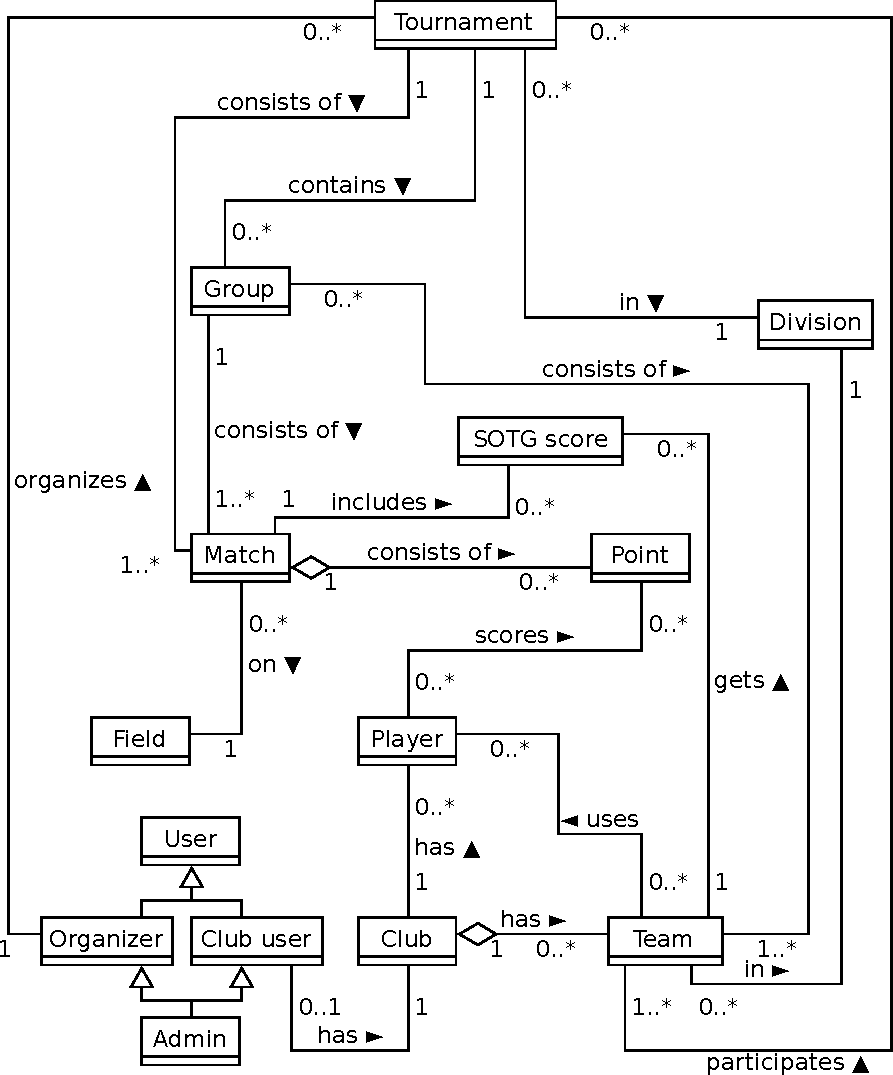
\includegraphics[width=130mm]{./images/domenovy-model.pdf}
\caption{Doménový model\label{overflow}}
\label{fig:domain_model}
\end{figure}


\begin{description}
  \item[Uživatel (user)]
  Uživatel je identifikován e-mailem a heslem nebo tokenem (více v sekci~\ref{sec:security}).
  Zároveň disponuje jednou ze tří rolí (\texttt{club}, \texttt{organizer} a~\texttt{admin}).
  \item[Oddíl (club)]
  Oddíl je logický prvek, který zastřešuje více týmů. Správu oddílu provádí klubový účet.
  \item[Tým (team)]
  Tým je vázán na oddíl. Jeho identifikátory jsou divize a stupeň týmu (např. A-tým).
  \item[Divize (division)]
  Kategorie, ve které se pořádají turnaje, nebo je složen tým. Například juniorská divize. % Například ženský tým je v divizi \texttt{women}.
  \item[Turnaj (tournament)]
    Turnaj může nabývat několika stavů (stavový diagram na~obrázku~\ref{fig:state_tournament}).
    Po vytvoření turnaje lze až do potvrzení (příznak \texttt{ready}) měnit týmy, které se turnaje zúčastní.
    Po něm mohou klubové účty odevzdávat soupisky za svoje týmy a na turnaji je možné aktivovat zápasy. Ve chvíli,
    kdy všechny týmy odevzdají svoje hodnocení SOTG a je známo finální pořadí týmů,
    lze turnaj ukončit (příznak \texttt{terminated}). Do~té~doby skryté výsledky hodnocení SOTG se stanou veřejnými.
    Turnaj je spravován administrátorem nebo uživatelem s rolí \texttt{organizer} (tzv.~organizátor).
    \begin{figure}[ht!]
      \centering
      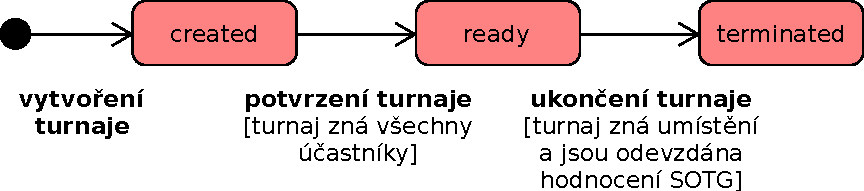
\includegraphics[width=110mm]{./images/stavovy-diagram-turnaj.pdf}
      \caption{Stavový diagram turnaje\label{overflow}}
      \label{fig:state_tournament}
    \end{figure}
  \item[Zápas (match)]
    Zápas má, stejně jako turnaj, tři stavy (obrázek~\ref{fig:state_match}). Akti\-vováním zápasu je umožněno zadat konečný výsledek
    nebo postupně vkládat jednotlivé body. Ukončením (příznak \texttt{terminated}) se konečný výsledek uloží a~následně se promítne
    v dalším postupu turnajem (vítězný tým posune do dalšího zápasu, týmům se přidá výhra ve skupině~apod.).
    \begin{figure}[ht!]
      \centering
      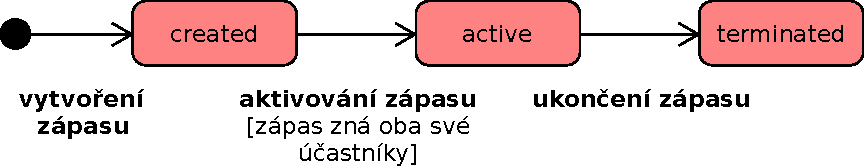
\includegraphics[width=110mm]{./images/stavovy-diagram-zapas.pdf}
      \caption{Stavový diagram zápasu\label{overflow}}
      \label{fig:state_match}
    \end{figure}
  \item[Bod (point)]
    Zápas je složen z několika bodů. Každý bod je záznamem o~skórování. Uchovává informaci, jaký hráč a komu nahrával.
    Zápas může být ukončen i bez jednotlivých bodů zadáním konečného skóre.
  \item[Skupina (group)]
    Jde o několik týmů, které hrají zápasy pouze mezi sebou. Po odehrání všech utkání ve skupině se podle pravidel určí pořadí a~na~jeho základě se týmy posunou turnajem dál.
  \item[Hřiště (field)]
    Zápas se musí někde hrát. K tomu slouží hřiště.
  \item[Hodnocení SOTG (SOTG score)]
    Po každém utkání musí tým ohodnotit soupeře hodnocením Spirit of the Game. Zjednodušeně jde o~číselné vyjádření na~stupnici od~0 do 20.
\end{description}

\subsection{Datový model}

Pro ujasnění entit a vazeb mezi nimi byl vhodný doménový model. Jeho konkrétní implementací je model datový.
Ten je dekomponován, tj. zbavení se M:N~vazeb, a oproti doménovému modelu obsahuje nové
(relační) objekty, včetně atributů. Kompletní datový model je dostupný v příloze~\ref{appendix:data_model}.

\section{Identifikace zdrojů}

Abychom mohli namapovat zdroje na konkrétní URI\footnote{Uniform Resource Identifier},
musíme nejprve jedno\-značně určit zdroje. Mnoho programátorů zde postupuje tak, že vychází
z~datového modelu a~použije prosté mapování \textit{tabulka = zdroj}.
Návrh je sice rychlý, ale nemusí být dostatečný. Navíc vytváří příliš těsnou vazbu mezi interní datovou reprezentací
a~logickou strukturou zdrojů. Zdroje v této práci vycházejí z doménového modelu.

\subsection{Základní typy zdrojů}

Podle~\cite{rest_vse} se zdroje dělí na tři základní typy:

\begin{description}
  \item[Dokument] Reprezentace jednoho konkrétního zdroje v určitém formátu.
  \item[Kolekce] Množina zdrojů stejného typu. Jedná se o skupiny samostných entit.
  \item[Kontroler] Nezávislé metody aplikace. Akce, které nelze vyjádřit pomocí standartních
  CRUD\footnote{Create, Read, Update, Delete - vytváření, čtení, úpravy a mazání} metod HTTP protokolu.
\end{description}

\subsection{Návrh URI}

Návrh se týká cesty v hierarchické části URI. Pro udržení kvality je doporučené se při návrhu držet několika zásad. Cesta by podle~\cite{rest_vse} měla:
    
\begin{itemize}
\item mít konzistentní a logickou strukturu
\item mít dobře znázorněnou hierarchickou strukturu
\item být nezávislá na zvolené technologii
\item transparentně používat HTTP metody a kódy
\item používat:
\begin{itemize}
\item jednotná čísla pro označení konkrétních zdrojů
\item množná čísla pro kolekce
\item slovesa pro kontrolery
\end{itemize}
\end{itemize}

\begin{figure}[ht!]
  \centering
  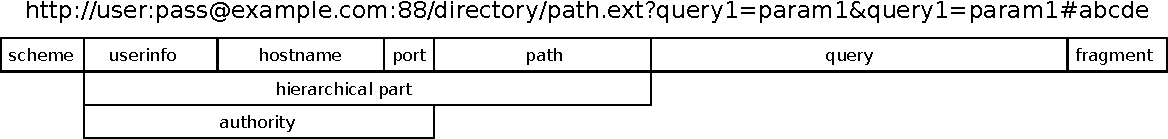
\includegraphics[width=130mm]{./images/uri.pdf}
  \caption{Jednotlivé komponenty URI; zdroj: autor na základě~\cite{uri}\label{overflow}}
\end{figure}

S těmito zásadami byl vytvořen následující návrh na mapování operací, které lze provádět nad zdroji.
Identifikátor značíme \texttt{\{id\}} nebo \texttt{\{ide\}} (druhý identifikátor je textový).
V cestách je vynechán prefix \texttt{/api}, který odděluje aplikační a dokumentační část.

\begin{itemize}
  \item \texttt{\textbf{/login}}
  \begin{itemize}
    \item \textbf{popis:} Přihlašuje uživatele. Po přihlášení vrátí přístupový token (více v sekci~\ref{sec:security}).
    \item \textbf{metoda:} POST
    \item \textbf{pokrývá:} UC3
  \end{itemize}
  \item \texttt{\textbf{/forgotten-password}}
  \begin{itemize}
    \item \textbf{popis:} Odešle nové náhodně vygenerované heslo na e-mail uživatele.
    \item \textbf{metoda:} POST
    \item \textbf{pokrývá:} UC4
  \end{itemize}
  \item \texttt{\textbf{/users}}
  \begin{itemize}
    \item \textbf{popis:} Slouží k vytváření nových uživatelů.
    \item \textbf{metoda:} POST
    \item \textbf{pokrývá:} UC2
  \end{itemize}
  \item \texttt{\textbf{/user/\{id\}}}
  \begin{itemize}
    \item \textbf{popis:} Spravuje konkrétního uživatele. Lze mu nastavit nový e-mail nebo~heslo.
    \item \textbf{metoda:} PUT
    \item \textbf{pokrývá:} UC21
  \end{itemize}
  \pagebreak
  \item \texttt{\textbf{/clubs}}
  \begin{itemize}
    \item \textbf{popis:} Kolekce oddílů.
    \item \textbf{metoda:} GET, POST
    \item \textbf{pokrývá:} UC5, UC6
  \end{itemize}
  \item \texttt{\textbf{/club/\{id\}}}
  \begin{itemize}
    \item \textbf{popis:} Operace nad konkrétním oddílem. Možnost uložit město a~zemi původu.
    \item \textbf{metoda:} GET, PUT, DELETE
    \item \textbf{pokrývá:} UC6, UC7, UC8
  \end{itemize}
  \item \texttt{\textbf{/club/\{id\}/players}}
  \begin{itemize}
    \item \textbf{popis:} Kolekce všech klubových hráčů.
    \item \textbf{metoda:} GET
    \item \textbf{pokrývá:} UC10
  \end{itemize}
  \item \texttt{\textbf{/club/\{id\}/teams}}
  \begin{itemize}
    \item \textbf{popis:} Kolekce všech týmů, které zastřešuje konkrétní oddíl.
    \item \textbf{metoda:} GET
    \item \textbf{pokrývá:} UC14
  \end{itemize}
  \item \texttt{\textbf{/players}}
  \begin{itemize}
    \item \textbf{popis:} Kolekce hráčů.
    \item \textbf{metoda:} GET, POST
    \item \textbf{pokrývá:} UC9, UC10
  \end{itemize}
  \item \texttt{\textbf{/player/\{id\}}}
  \begin{itemize}
    \item \textbf{popis:} Operace nad konkrétním hráčem.
    \item \textbf{metoda:} GET, PUT, DELETE
    \item \textbf{pokrývá:} UC10, UC11, UC12
  \end{itemize}
  \pagebreak
  \item \texttt{\textbf{/teams/}}
  \begin{itemize}
    \item \textbf{popis:} Kolekce týmů.
    \item \textbf{metoda:} GET, POST
    \item \textbf{pokrývá:} UC13, UC14
  \end{itemize}
  \item \texttt{\textbf{/team/\{id\}}}
  \begin{itemize}
    \item \textbf{popis:} Operace nad konkrétním týmem.
    \item \textbf{metoda:} GET, PUT, DELETE
    \item \textbf{pokrývá:} UC14, UC15, UC16
  \end{itemize}
  \item \texttt{\textbf{/divisions}}
  \begin{itemize}
    \item \textbf{popis:} Kolekce divizí.
    \item \textbf{metoda:} GET
  \end{itemize}
  \item \texttt{\textbf{/tournaments}}
  \begin{itemize}
    \item \textbf{popis:} Kolekce turnajů, kterou lze filtrovat pomocí pěti různých parametrů.
    \item \textbf{metoda:} GET, POST
    \item \textbf{pokrývá:} UC17, UC19
  \end{itemize}
  \item \texttt{\textbf{/tournament/\{id\}}}
  \begin{itemize}
    \item \textbf{popis:} Správa turnaje. Možnost turnaji upravit příznaky \texttt{ready} a~\texttt{terminated}.
    \item \textbf{metoda:} GET, PUT
    \item \textbf{pokrývá:} UC18, UC19
  \end{itemize}
  \item \texttt{\textbf{/tournament/\{id\}/standings}}
  \begin{itemize}
    \item \textbf{popis:} Zobrazuje výsledné pořadí týmů na turnaji, včetně kategorie SOTG.
    \item \textbf{metoda:} GET
    \item \textbf{pokrývá:} UC20
  \end{itemize}
  \item \texttt{\textbf{/tournament/\{id\}/players}}
  \begin{itemize}
    \item \textbf{popis:} Slouží pro správu soupisek na turnaji.
    \item \textbf{metoda:} GET, POST, DELETE
    \item \textbf{pokrývá:} UC21, UC22, UC23
  \end{itemize}
  \pagebreak
  \item \texttt{\textbf{/tournament/\{id\}/teams}}
  \begin{itemize}
    \item \textbf{popis:} Slouží pro správu týmů na turnaji.
    \item \textbf{metoda:} GET, PUT
  \end{itemize}
  \item \texttt{\textbf{/tournament/\{id\}/matches}}
  \begin{itemize}
    \item \textbf{popis:} Kolekce zápasů, kterou lze filtrovat pomocí šesti různých parametrů.
    \item \textbf{metoda:} GET
    \item \textbf{pokrývá:} UC25\\
  \end{itemize}
  \item \texttt{\textbf{/tournament/\{id\}/groups}}
  \begin{itemize}
    \item \textbf{popis:} Kolekce skupin.
    \item \textbf{metoda:} GET
    \item \textbf{pokrývá:} UC24
  \end{itemize}
  \item \texttt{\textbf{/tournament/\{id\}/group/\{ide\}}}
  \begin{itemize}
    \item \textbf{popis:} Konkrétní skupina.
    \item \textbf{metoda:} GET
    \item \textbf{pokrývá:} UC24
  \end{itemize}
  \item \texttt{\textbf{/tournament/\{id\}/spirits}}
  \begin{itemize}
    \item \textbf{popis:} Kolekce všech hodnocení SOTG. Možnost filtrovat hodnocení pro jeden konkrétní tým.
    \item \textbf{metoda:} GET
    \item \textbf{pokrývá:} UC31
  \end{itemize}
  \item \texttt{\textbf{/tournament/\{id\}/missing-spirits}}
  \begin{itemize}
    \item \textbf{popis:} Seznam týmů, které hodnocení SOTG neodevzdaly.
    \item \textbf{metoda:} GET
    \item \textbf{pokrývá:} UC32
  \end{itemize}
  \item \texttt{\textbf{/match/\{id\}}}
  \begin{itemize}
    \item \textbf{popis:} Správa utkání.
    \item \textbf{metoda:} GET, PUT, 
    \item \textbf{pokrývá:} UC25, UC26
  \end{itemize}
  \pagebreak
  \item \texttt{\textbf{/match/\{id\}/points}}
  \begin{itemize}
    \item \textbf{popis:} Zobrazuje detailní popis zápasu. Konkrétně jeho odehrané body seřazené chronologicky.
      Dál poskytuje ukládání nových bodů a úpravu stávajících (například změna hráče, který skóroval).
    \item \textbf{metoda:} GET, POST, PUT, DELETE
    \item \textbf{pokrývá:} UC25
  \end{itemize}
  \item \texttt{\textbf{/match/\{id\}/spirits}}
  \begin{itemize}
    \item \textbf{popis:} Vrátí detail jednoho zápasu včetně hodnocení SOTG obou týmů. Kromě toho umožňuje odevzdat hodnocení SOTG.
    \item \textbf{metoda:} GET, POST, PUT
    \item \textbf{pokrývá:} UC25, UC29, UC30
  \end{itemize}
\end{itemize}